\headline{{\textbf{\Large\sffamily Japanese Growing Techniques for Mame}}\\
          {\textbf{\large\sffamily By David Cheshire}}}
\label{2025-04-techniques}
\noindent
% David Cheshire (David Cheshire Nurseries) opened his talk by observing a trend among enthusiasts---moving towards smaller trees, or \textit{mame bonsai}. His interest in these miniature specimens led him to study specialised techniques in Japan, particularly from nurseries focusing on compact, naturally styled trees. He emphasised that traditional Japanese bonsai (\textit{noe\--uchi}, meaning ``natural bonsai'') prioritises slow, organic growth over the modern commercial approach, which favours rapid development and dramatic features like thick trunks.  
% The core difference lies in patience: traditional methods mimic how trees grow in harsh wild conditions---think of a seed lodged in a mountain crevice, surviving on minimal soil and water. These trees develop gnarled bark and compact forms over decades, sometimes centuries. Modern techniques, however, are designed for efficiency, often sacrificing longevity for quicker results.
% \medskip
% \topic{\large{Traditional Slow-Growth Techniques}
% \topic{Potting and Root Management}
% \noindent
% For \textit{mame bonsai}, David stressed starting with seedlings in \textbf{tiny pots}---no larger than a fist---for the first 5–6 years. The goal isn't vigorous growth but survival, allowing the bark to harden naturally. Repotting is done incrementally into slightly larger containers, \textbf{without root pruning}. Instead, the tree is raised higher in the pot over time, letting surface roots emerge and thicken, creating the illusion of age.  
% \medskip
% \topic{Environmental Conditioning}
% \noindent
% Trees are ``programmed'' to thrive in austerity:  
% \begin{itemize}
%     \item \textbf{Watering}: Minimal irrigation trains roots to seek moisture, preventing reliance on constant care.  
%     \item \textbf{Nutrients}: Sparingly applied to avoid lush, unsustainable growth.  
% \end{itemize}
% This mimics nature, where stunted trees outlive fast-grown ones. A 45-year-old pine shown at the talk had a trunk no thicker than a pencil but displayed deeply fissured bark---proof of this method's effectiveness.  
% \medskip
% \topic{Shaping Without Wiring}
% \noindent
% Instead of wire, David demonstrated how sunlight manipulation shapes trees. For example:  
% \begin{itemize}
%     \item Tilting a pot forces branches to grow toward the light, creating movement.  
%     \item A red pine in the talk had never been wired; its curves resulted from decades of strategic repositioning.  
% \end{itemize}
% Branches are allowed to die back naturally, adding character---a stark contrast to the ``perfect'' aesthetics of modern bonsai.  
% \topic{\large{Fast-Growth Methods and Their Trade-Offs}}
% \topic{Sacrificial Branch Technique}
% \noindent
% For quicker results, David showcased a Japanese maple grown in coarse volcanic grit. To thicken the trunk, a \textbf{sacrificial branch} was partially removed:  
% \begin{itemize}
%     \item The underside was carved out, leaving a thin connection to draw sap.  
%     \item Once callus tissue half-covered the wound, the branch was fully removed, ensuring smooth healing.  
% \end{itemize}
% While effective, such methods risk internal rot, limiting the tree's lifespan to 40–50 years.  
% \medskip
% \topic{Grafting for Speed}
% \noindent
% \begin{itemize}
%     \item \textbf{Vigorous Rootstock}: Fast-growing species (e.g., \textit{San Jose juniper}) form trunks quickly.  
%     \item \textbf{Desired Foliage}: Slower varieties (e.g., \textit{Itoigawa juniper}) are grafted onto the established trunk.  
% \end{itemize}
% David noted that grafts must dominate early---if the rootstock's foliage isn't removed promptly, it can outcompete the grafted branches.  
% \medskip
% \topic{\large{Species-Specific Strategies}}
% \topic{Zelkova: The Tied-Branch Trick}
% \noindent
% Japanese elms (\textit{zelkova}) often have tightly clustered crowns in maturity. To replicate this in \textit{mame} sizes:  
% \begin{itemize}
%     \item Young branches are \textbf{bound together with wire} for months, encouraging upright growth.  
%     \item Once released, they retain a compact, broom-like silhouette.  
% \end{itemize}
% \medskip
% \topic{Elms: Propagation Secrets}
% \noindent
% Elms (\textit{Ulmus}) excel for \textit{mame} projects due to their adaptability:  
% \begin{itemize}
%     \item \textbf{Cuttings}: Taken from older, slower-growing side shoots (not vigorous tips) for compactness.  
%     \item \textbf{Winged Varieties}: Some elms develop corky bark ``wings''---David hunts for these rare traits to propagate.  
% \end{itemize}
% \medskip
% \topic{Pines: Embracing Seasonality}
% \noindent
% David urged attendees to appreciate seasonal changes:  
% \begin{itemize}
%     \item Yellowing autumn needles shouldn't be immediately plucked---their colour adds depth.  
%     \item Slow-grown pines develop finer needles and denser foliage over time.  
% \end{itemize}
% \medskip
% \topic{\large{Climate Adaptation: UK Challenges}}
% \topic{Humidity and Watering}
% \noindent
% \begin{itemize}
%     \item \textbf{Summer}: UK air is drier than Japan's. David uses gravel trays and brief sprinkler bursts to boost humidity \textbf{without overwatering roots}.  
%     \item \textbf{Winter}: Wet cold promotes fungus. Trees are kept drier, with shelter from relentless rain.  
% \end{itemize}
% \medskip
% \topic{Light and Heat Management}
% \noindent
% Small pots heat rapidly in direct sun. Solutions:  
% \begin{itemize}
%     \item \textbf{Shade Cloth}: Filters intense midday light.  
%     \item \textbf{Grouping Trees}: Creates a self-shading microclimate.  
% \end{itemize}
% \medskip
% \topic{\large{Nursery Practices and Personal Insights}}
% \topic{Propagation Philosophy}
% \noindent
% \begin{itemize}
%     \item \textbf{High Volume}: Grow many seedlings---expect 50\% losses, as in nature. 
%     \item \textbf{Selection}: Keep only the strongest, most adaptable trees.  
% \end{itemize}
% \medskip
% \topic{Conclusion: Patience as the Core Principle}
% \noindent
% Whether adopting traditional \textit{noe-uchi} or modern shortcuts, David's message was clear: bonsai is a dialogue with nature. \textit{Mame} bonsai distills this into its purest form---where every year of patience is etched into the bark of a tree that fits in your palm.  
% QWERTY
% ASDFGH
% ZXCVBN
David Cheshire (\href{https://www.davidcheshirenurseries.co.uk}{David Cheshire Nurseries}) delivered an insightful talk on the art of growing Mame bonsai, sharing his extensive knowledge and practical experience. His discussion covered a wide range of topics, including environmental conditions, watering techniques, species selection, and propagation methods. His advice is particularly valuable for those looking to cultivate Mame bonsai successfully in the UK's climate. 

\medskip

\topic{Understanding the Climate Challenges}
\noindent
While the UK is often considered a wet country, David pointed out that it actually experiences low humidity during the summer months. This discrepancy between wet winters and dry summers creates specific challenges for bonsai growers. The combination of wet and cold conditions in winter promotes fungal growth and root rot, while hot and dry summers can lead to dehydration if not managed correctly.

The key challenge is maintaining an optimal moisture balance throughout the year. Overwatering in summer is a common mistake, as Mame bonsai, due to their small pots, dry out quickly when exposed to direct sunlight. David stressed that if the environment is managed correctly---providing shade and maintaining humidity around the trees---watering once a day is usually sufficient. He recommended placing gravel trays beneath benches or using sprinklers that mist for just a few minutes to boost humidity without over\-saturating the soil.

\medskip

\topic{Watering Strategies and Environmental Control}
\noindent
David discussed the importance of understanding how Mame bonsai dry out. A small pot exposed to direct sunlight can become excessively hot within ten minutes, leading to rapid evaporation. The key to managing this is to create a shaded environment with high humidity. 

In his nursery, David uses sprinklers to maintain humidity rather than for direct watering, as different tree species and pot sizes dry out at different rates. Instead, he visually inspects each tree to determine its watering needs. A well\--designed environment, with shade and controlled humidity, ensures trees remain healthy without excessive watering.

\medskip

\topic{Zelkova Bonsai: Structure and Training}
\noindent
David highlighted an interesting characteristic of Zelkova bonsai (a species commonly used in Japan). Unlike most bonsai species, which are trained to spread their branches, mature Zelkova trees naturally grow with a tight, upright branch structure. This natural growth pattern is essential to creating an authentic broom\--style appearance.

The Japanese approach to training Zelkova involves tying the branches together at the apex for a few months, which helps recreate the appearance of mature trees. David emphasised how this technique contrasts with standard bonsai training methods, making it an intriguing and unique aspect of Zelkova cultivation.

\medskip

\topic{Ulmus Bonsai: Rapid Growth and Development}
\noindent
David praised the Ulmus species (Elms) for their ability to develop quickly into impressive Mame bonsai. With regular pruning, their leaves can be kept remarkably small, creating a refined and mature appearance within five years. Their vigorous growth makes them a rewarding species for bonsai enthusiasts who wish to see significant development in a short period.

He described a specific Ulmus specimen he acquired in Japan, valued for its unique bark and distinctive winged growth on its branches. He plans to propagate from this tree, cutting branches to create numerous Mame bonsai. Given that Elms root easily from cuttings, he sees great potential in this species for Mame cultivation.

\medskip

\topic{Understanding Tree Age in Bonsai}
\noindent
One of the intriguing points David raised was the question of a tree's true age. He explained that when a bonsai is grown from a cutting taken from an older tree, it retains some characteristics of its parent. For example, a cutting from a ten\--year\--old branch may develop much faster than a seedling, raising the question: is it a one\--year\--old tree or a ten\--year\--old tree? 

Similarly, cuttings from flowering trees tend to retain their flowering characteristics, allowing bonsai growers to produce flowering specimens much more quickly than if they had grown the tree from seed.

\medskip

\topic{Selecting the Right Cuttings for Bonsai}
\noindent
David provided an important insight into the selection of cuttings for bonsai cultivation. He advised against using vigorous leader shoots from a parent tree, as these tend to produce long, fast\--growing extensions, which are not ideal for compact Mame bonsai. Instead, he recommended selecting weaker side branches, which naturally develop into more compact, finely branched trees.

This principle applies to both deciduous and coniferous species. Taking cuttings from side branches results in trees with shorter internodes and more refined growth, making them more suitable for bonsai.

\medskip

\topic{Propagation Techniques and Genetic Considerations}
\noindent
David discussed the unpredictable nature of propagation, noting that genetic and environmental factors both play a role in how a cutting develops. He pointed out that some characteristics---such as the winged bark of certain Elms---may be influenced more by environmental factors than genetics. Even if a parent tree displays a particular trait, its cuttings may not necessarily exhibit the same features.

In hedgerows, for example, trees frequently pruned by farmers often develop interesting characteristics, such as winged bark or compact growth habits. These traits may be a response to environmental stress rather than purely genetic inheritance.

\medskip

\begin{figure*}[!p]
\centering
\begin{minipage}[b]{.47\textwidth}
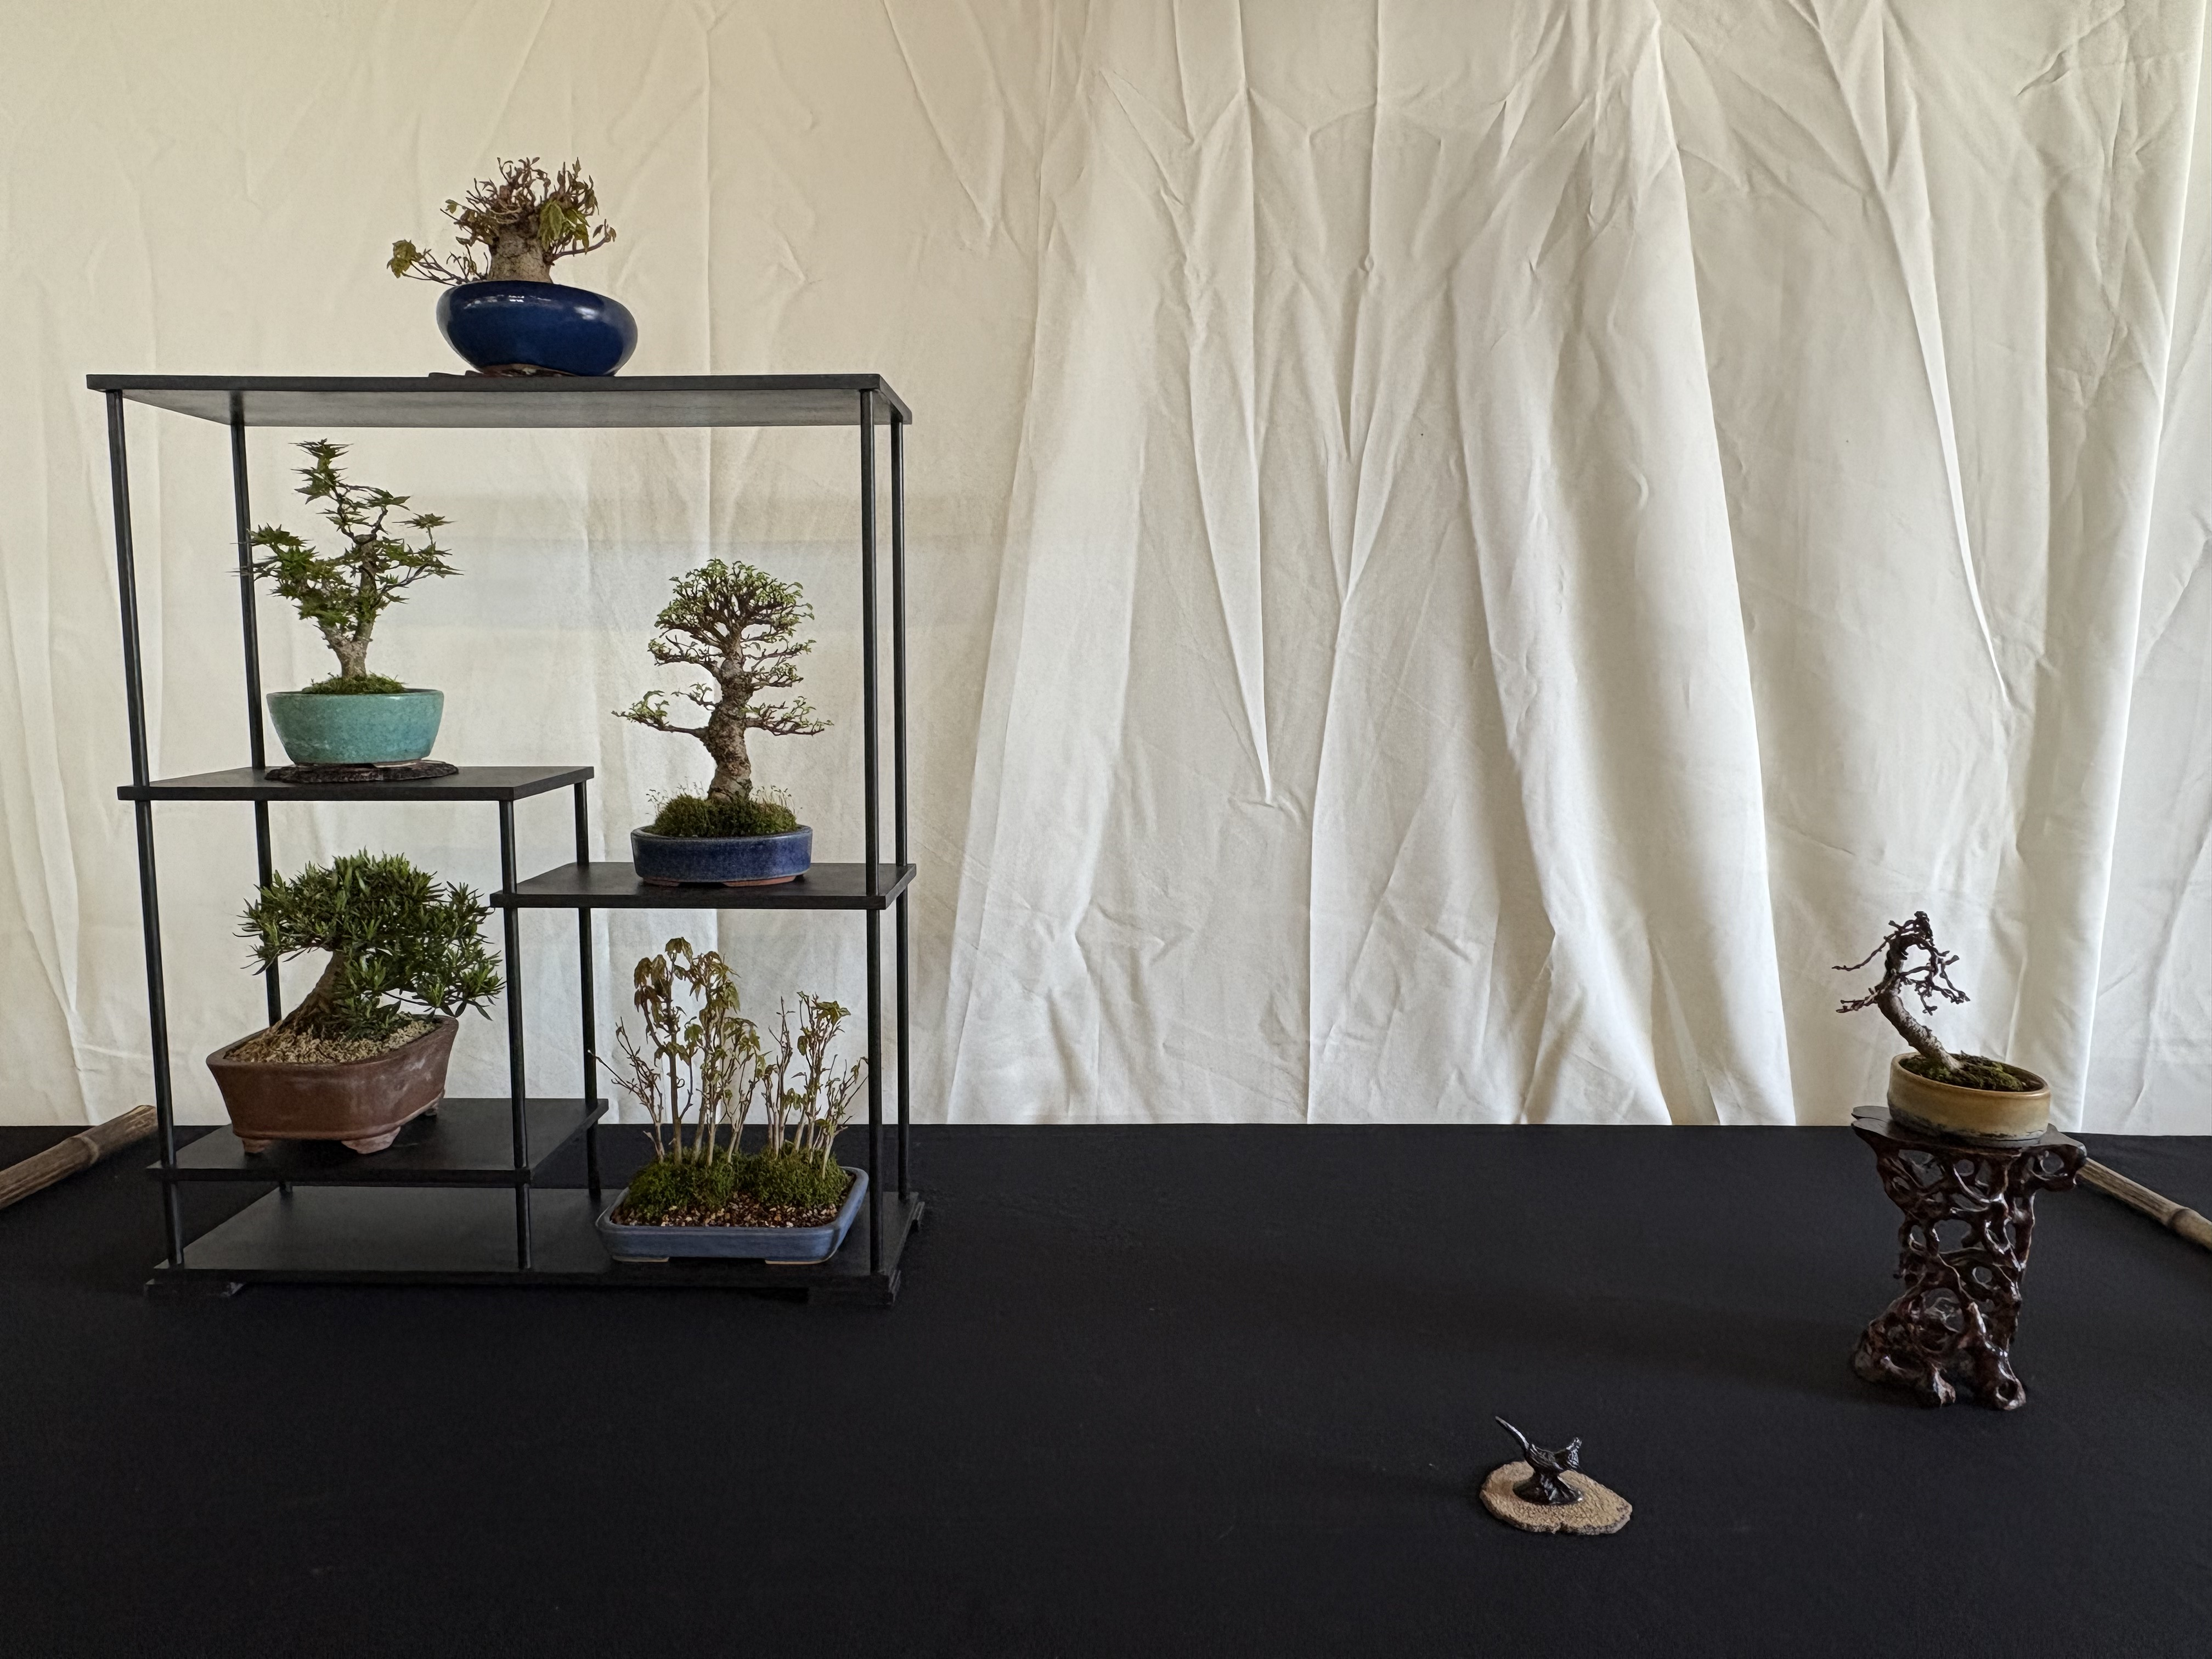
\includegraphics[width=1.0\textwidth]{2025_04/res/display_13.jpeg}
% \centerline{\emph{David's Hawthorn.}}
\end{minipage}\qquad
\begin{minipage}[b]{.47\textwidth}
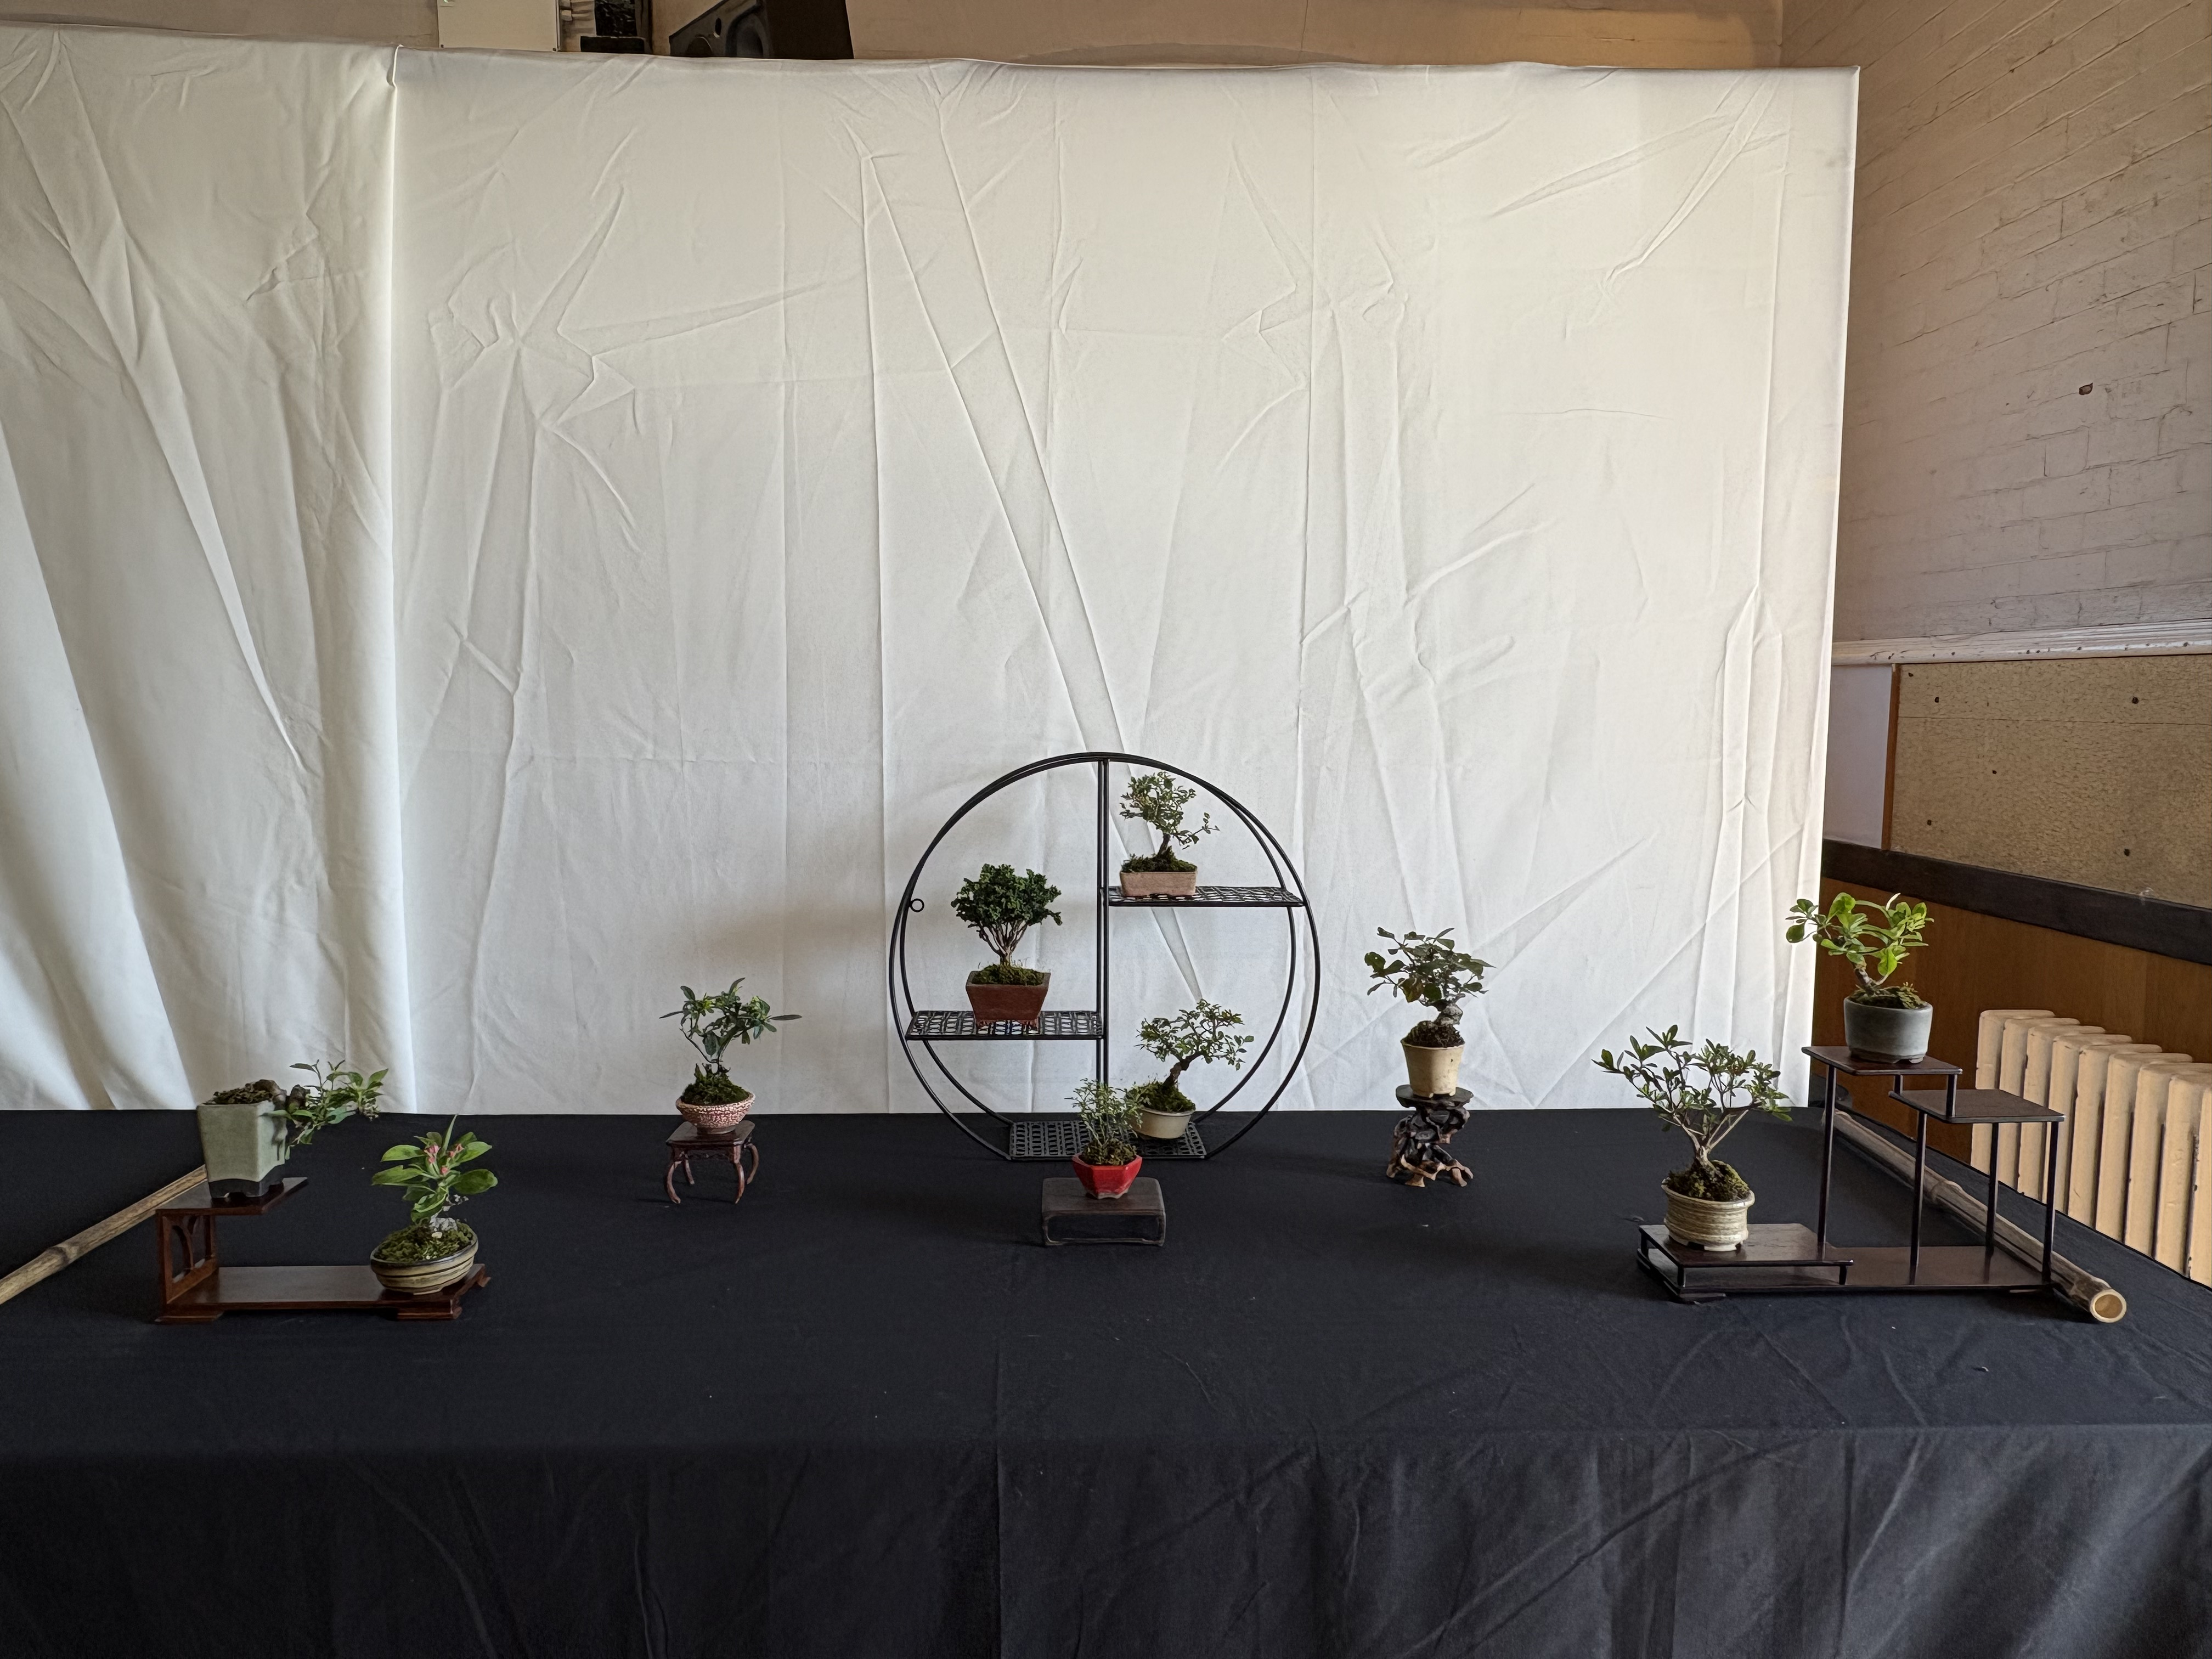
\includegraphics[width=1.0\textwidth]{2025_04/res/display_14.jpeg}
% \centerline{\emph{Nick's Privet.}}
\end{minipage}
\medskip

\begin{minipage}[b]{.47\textwidth}
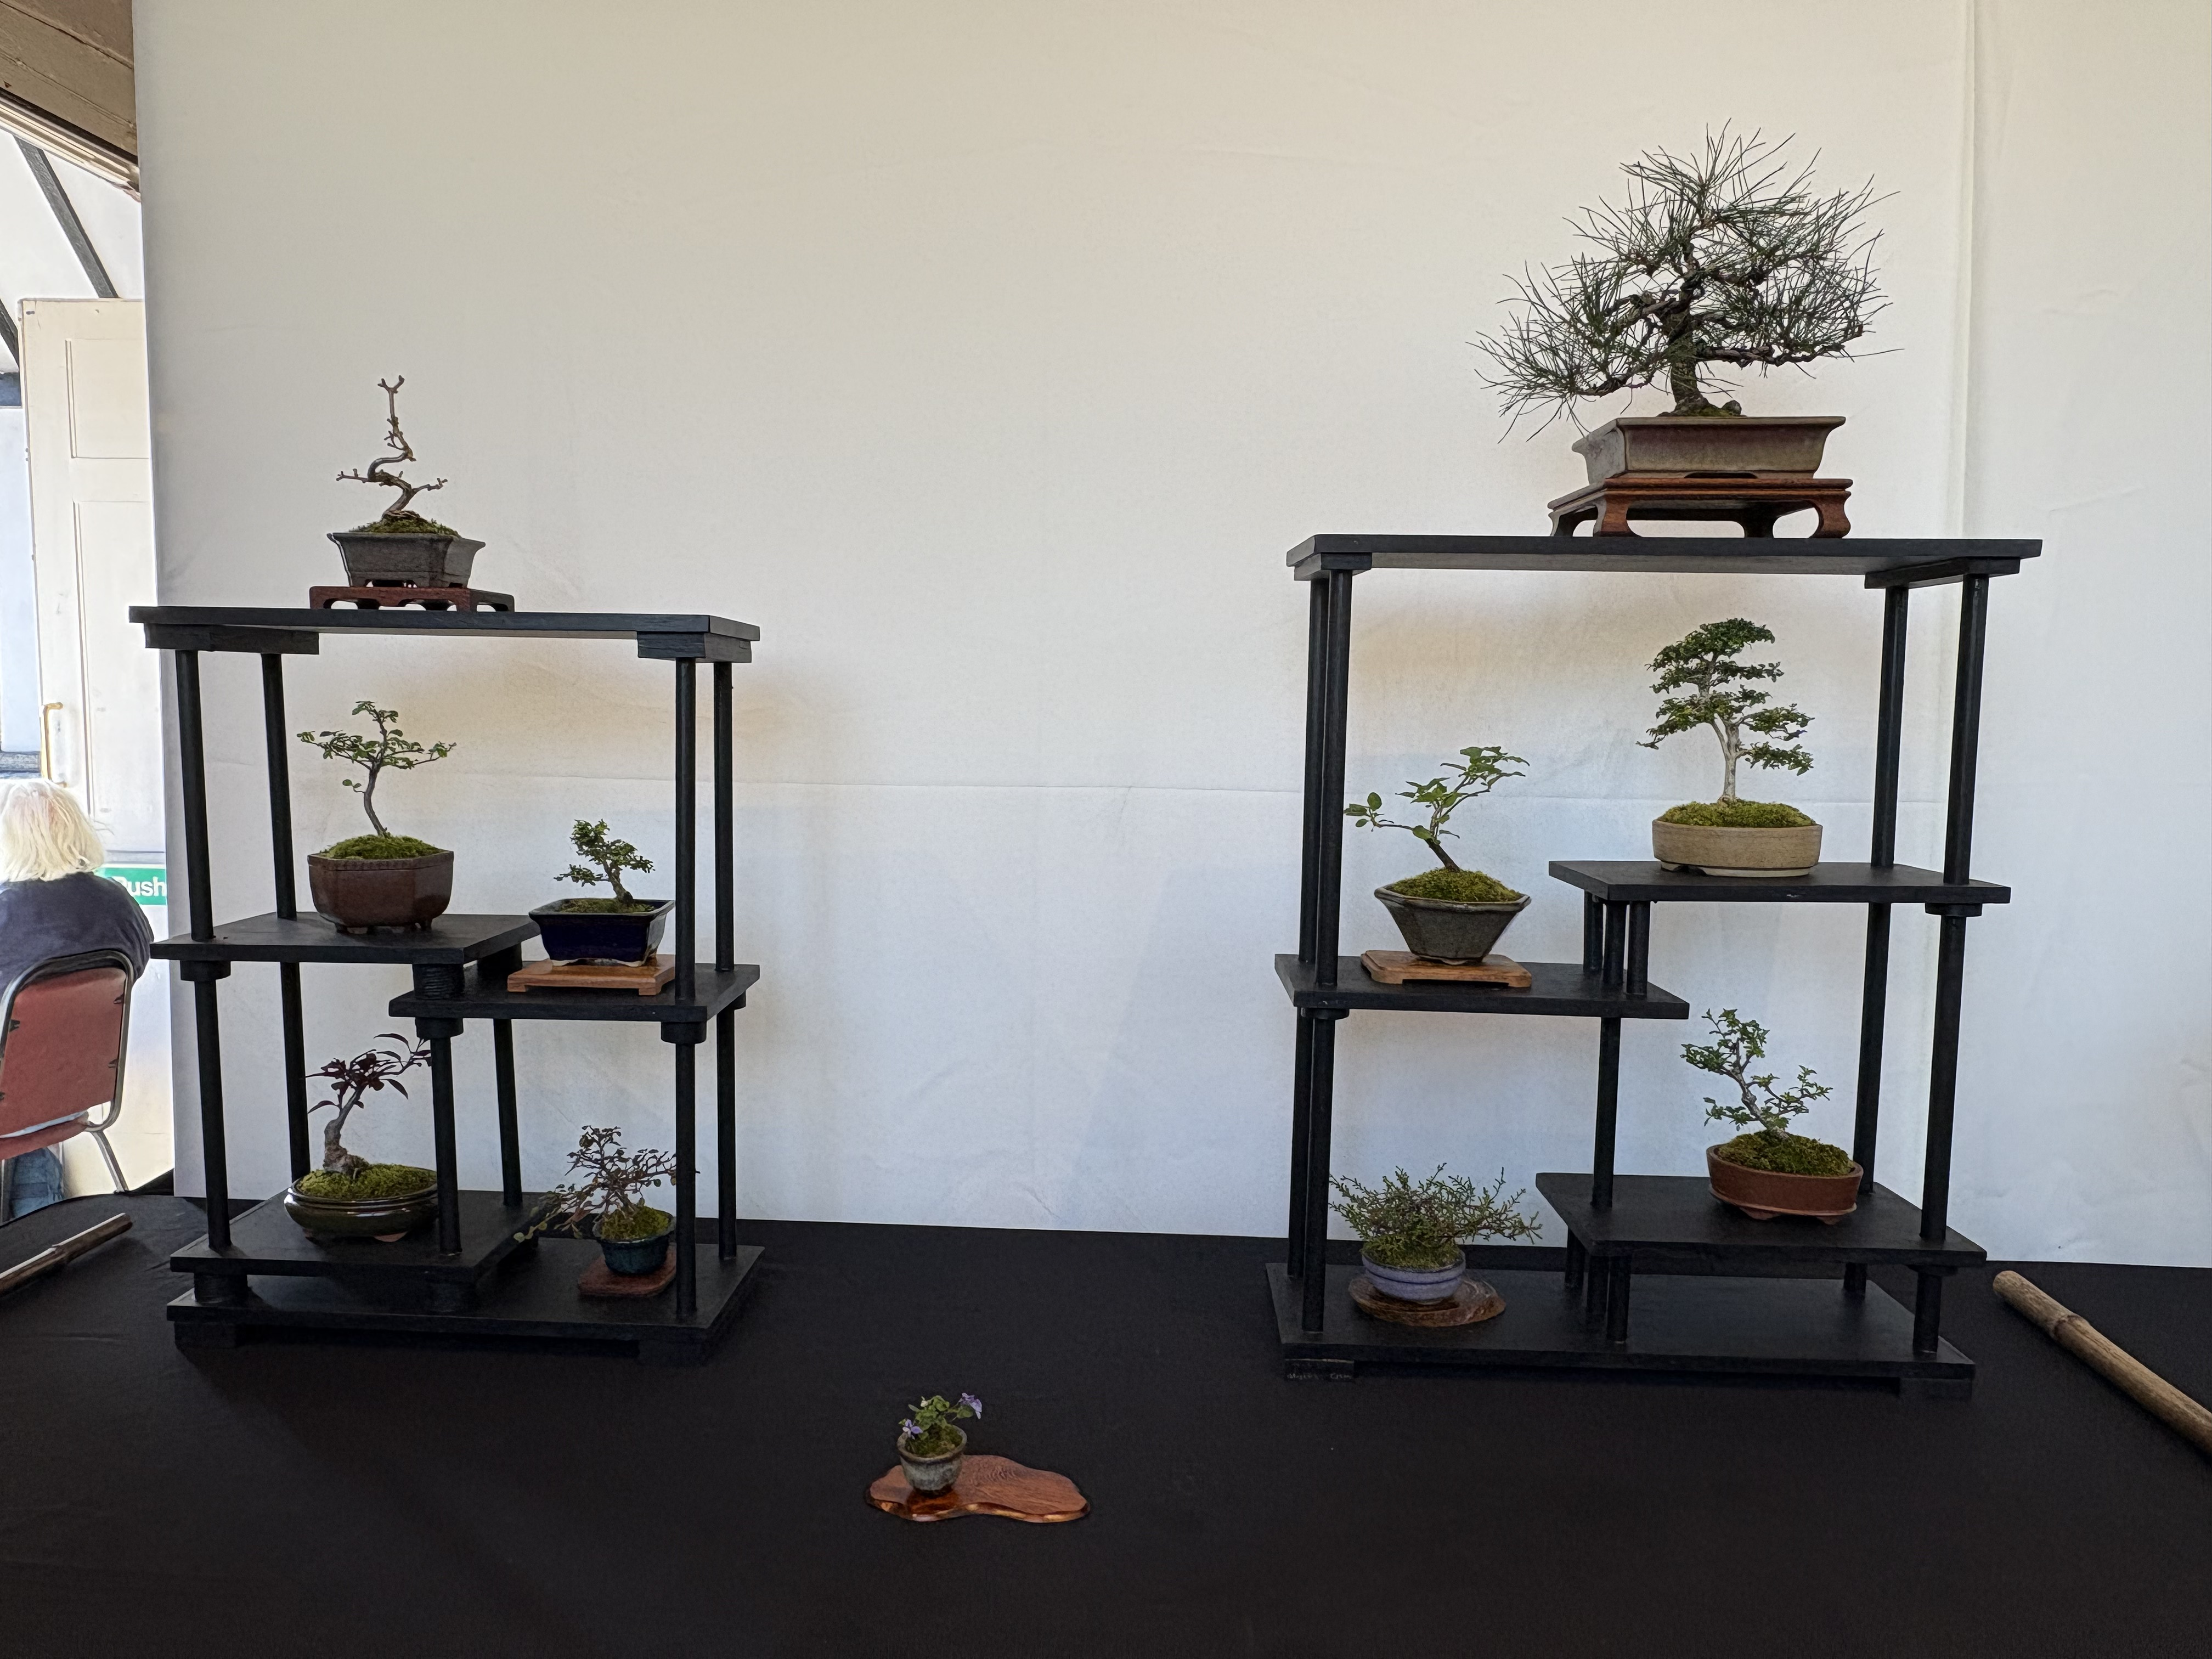
\includegraphics[width=1.0\textwidth]{2025_04/res/display_15.jpeg}
% \centerline{\emph{Brendan's Yew.}}
\end{minipage}\qquad
\begin{minipage}[b]{.47\textwidth}
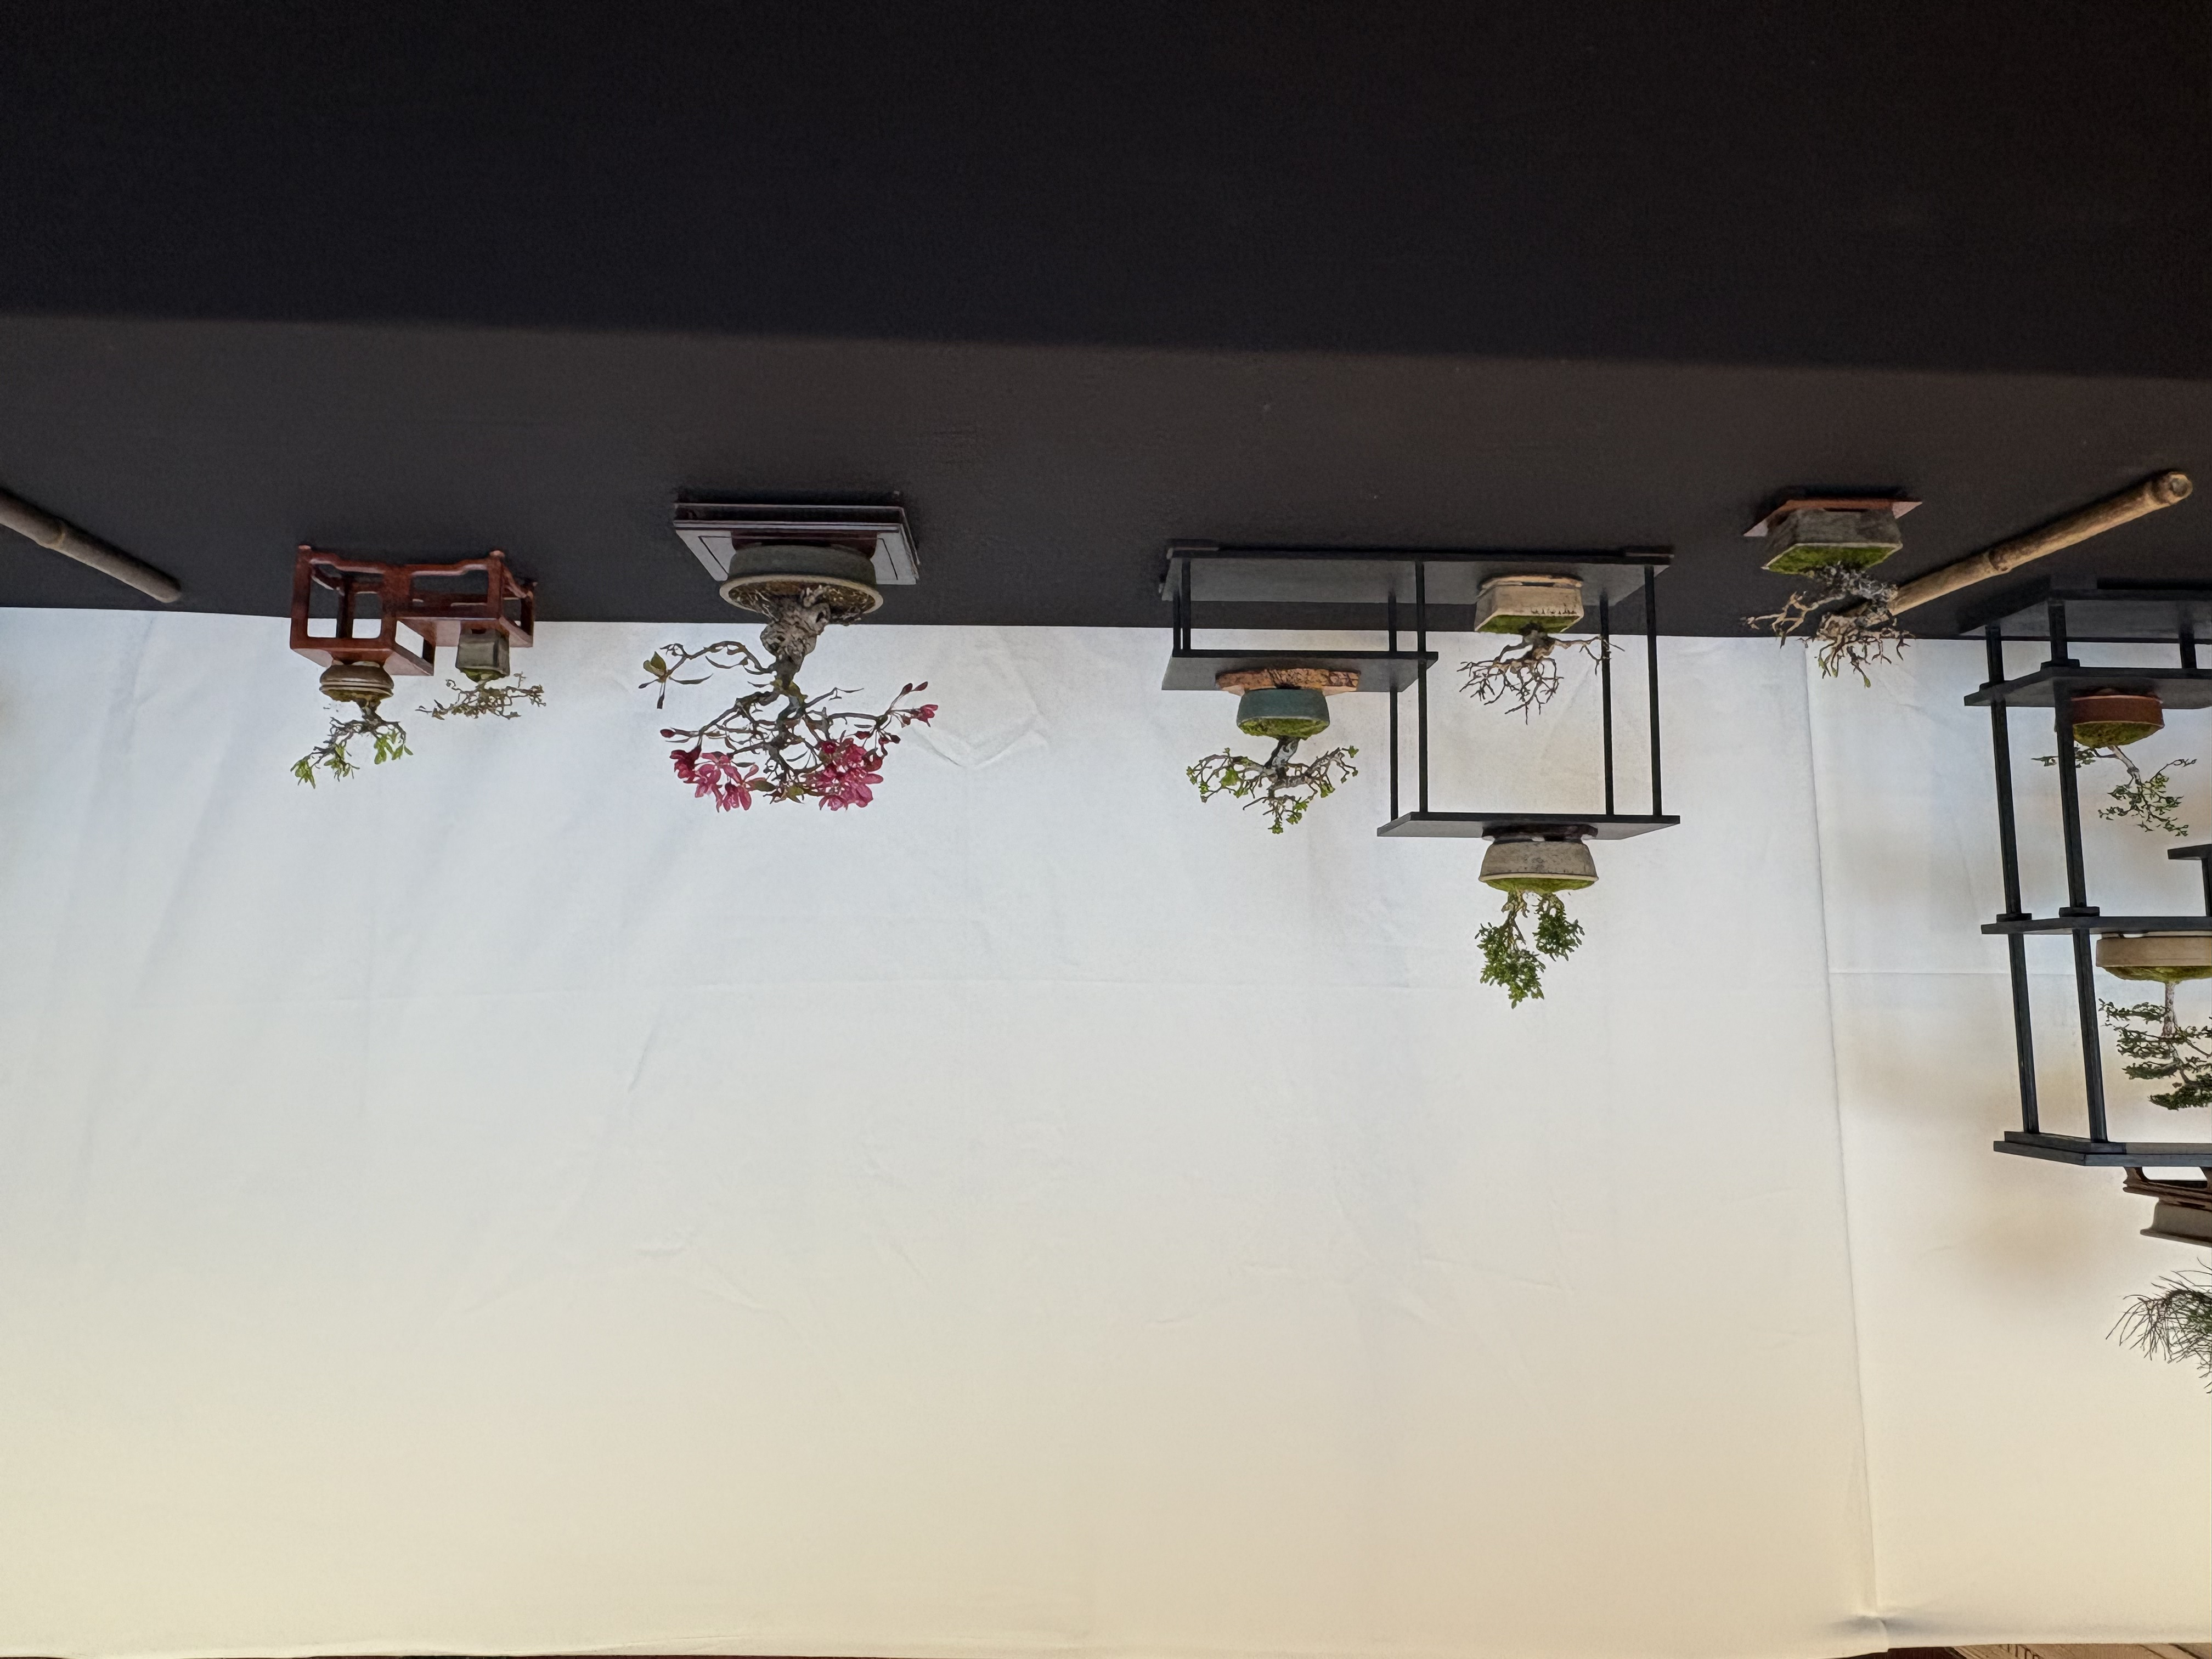
\includegraphics[angle=180,origin=c,width=1.0\textwidth]{2025_04/res/display_16.jpeg}
% \centerline{\emph{Tony's Hawthorn.}}
\end{minipage}
\medskip

\begin{minipage}[b]{.47\textwidth}
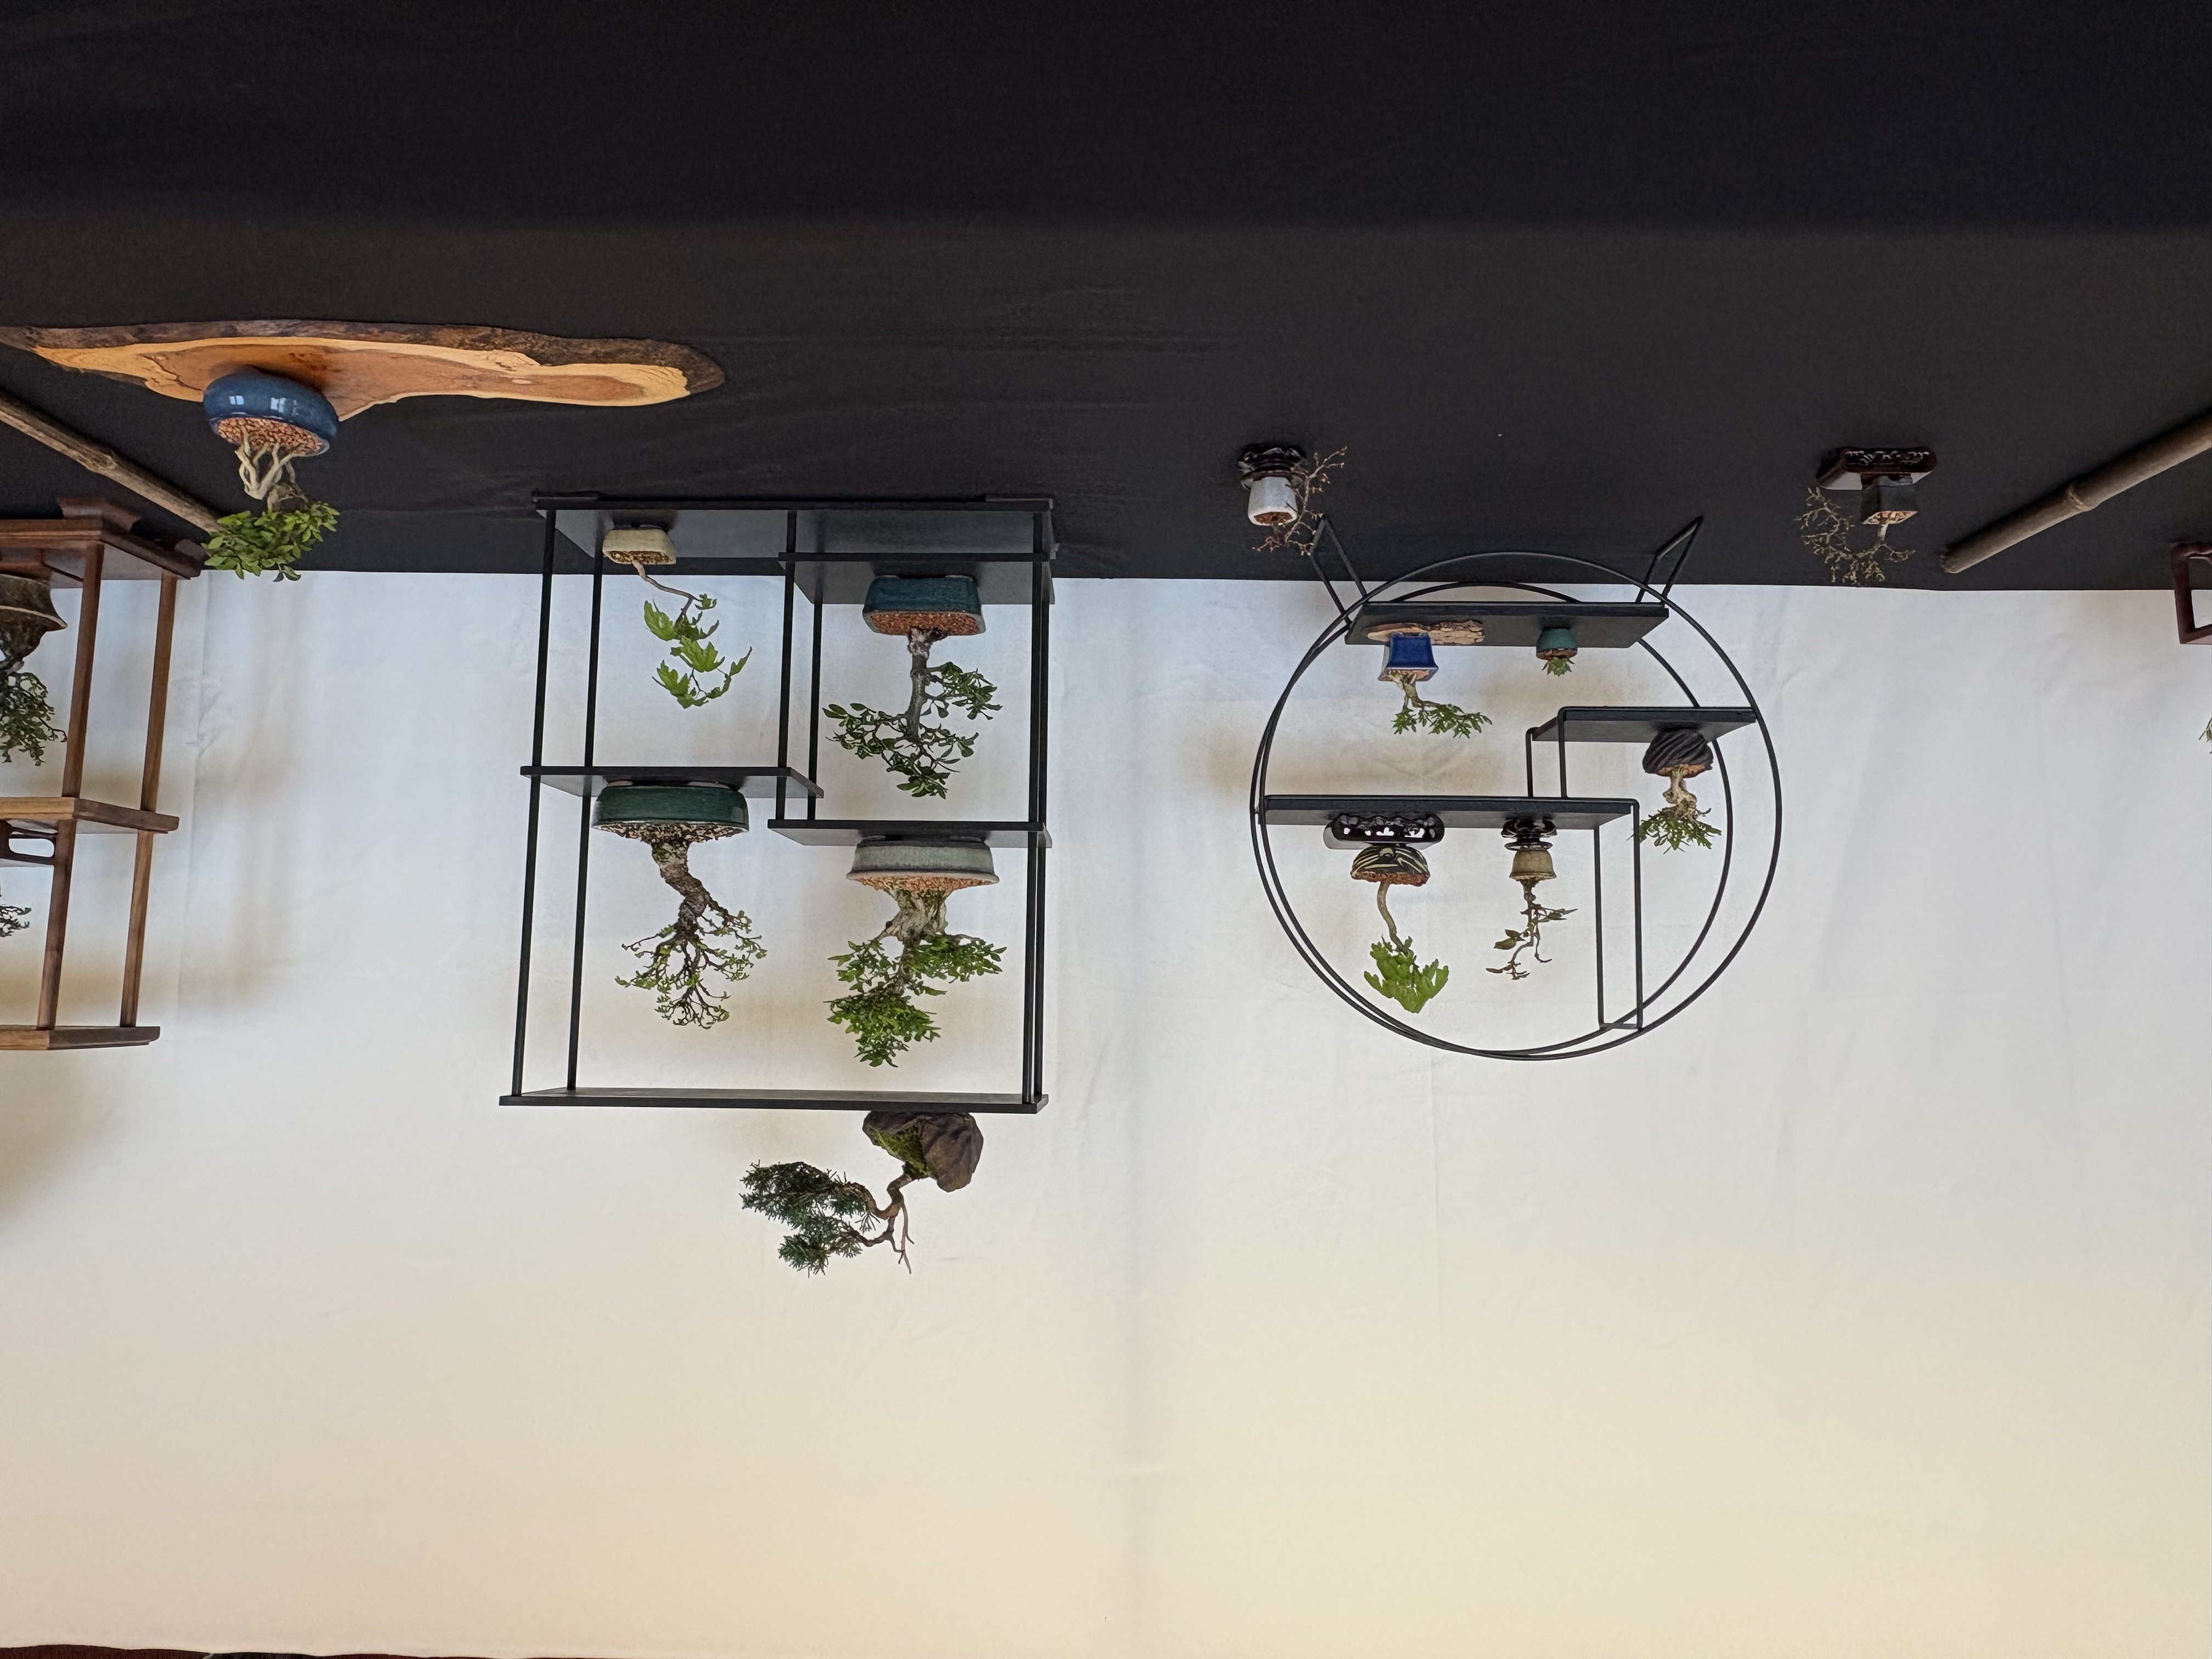
\includegraphics[angle=180,origin=c,width=1.0\textwidth]{2025_04/res/display_17.jpeg}
% \centerline{\emph{Terry's American Sweetgum.}}
\end{minipage}\qquad
\begin{minipage}[b]{.47\textwidth}
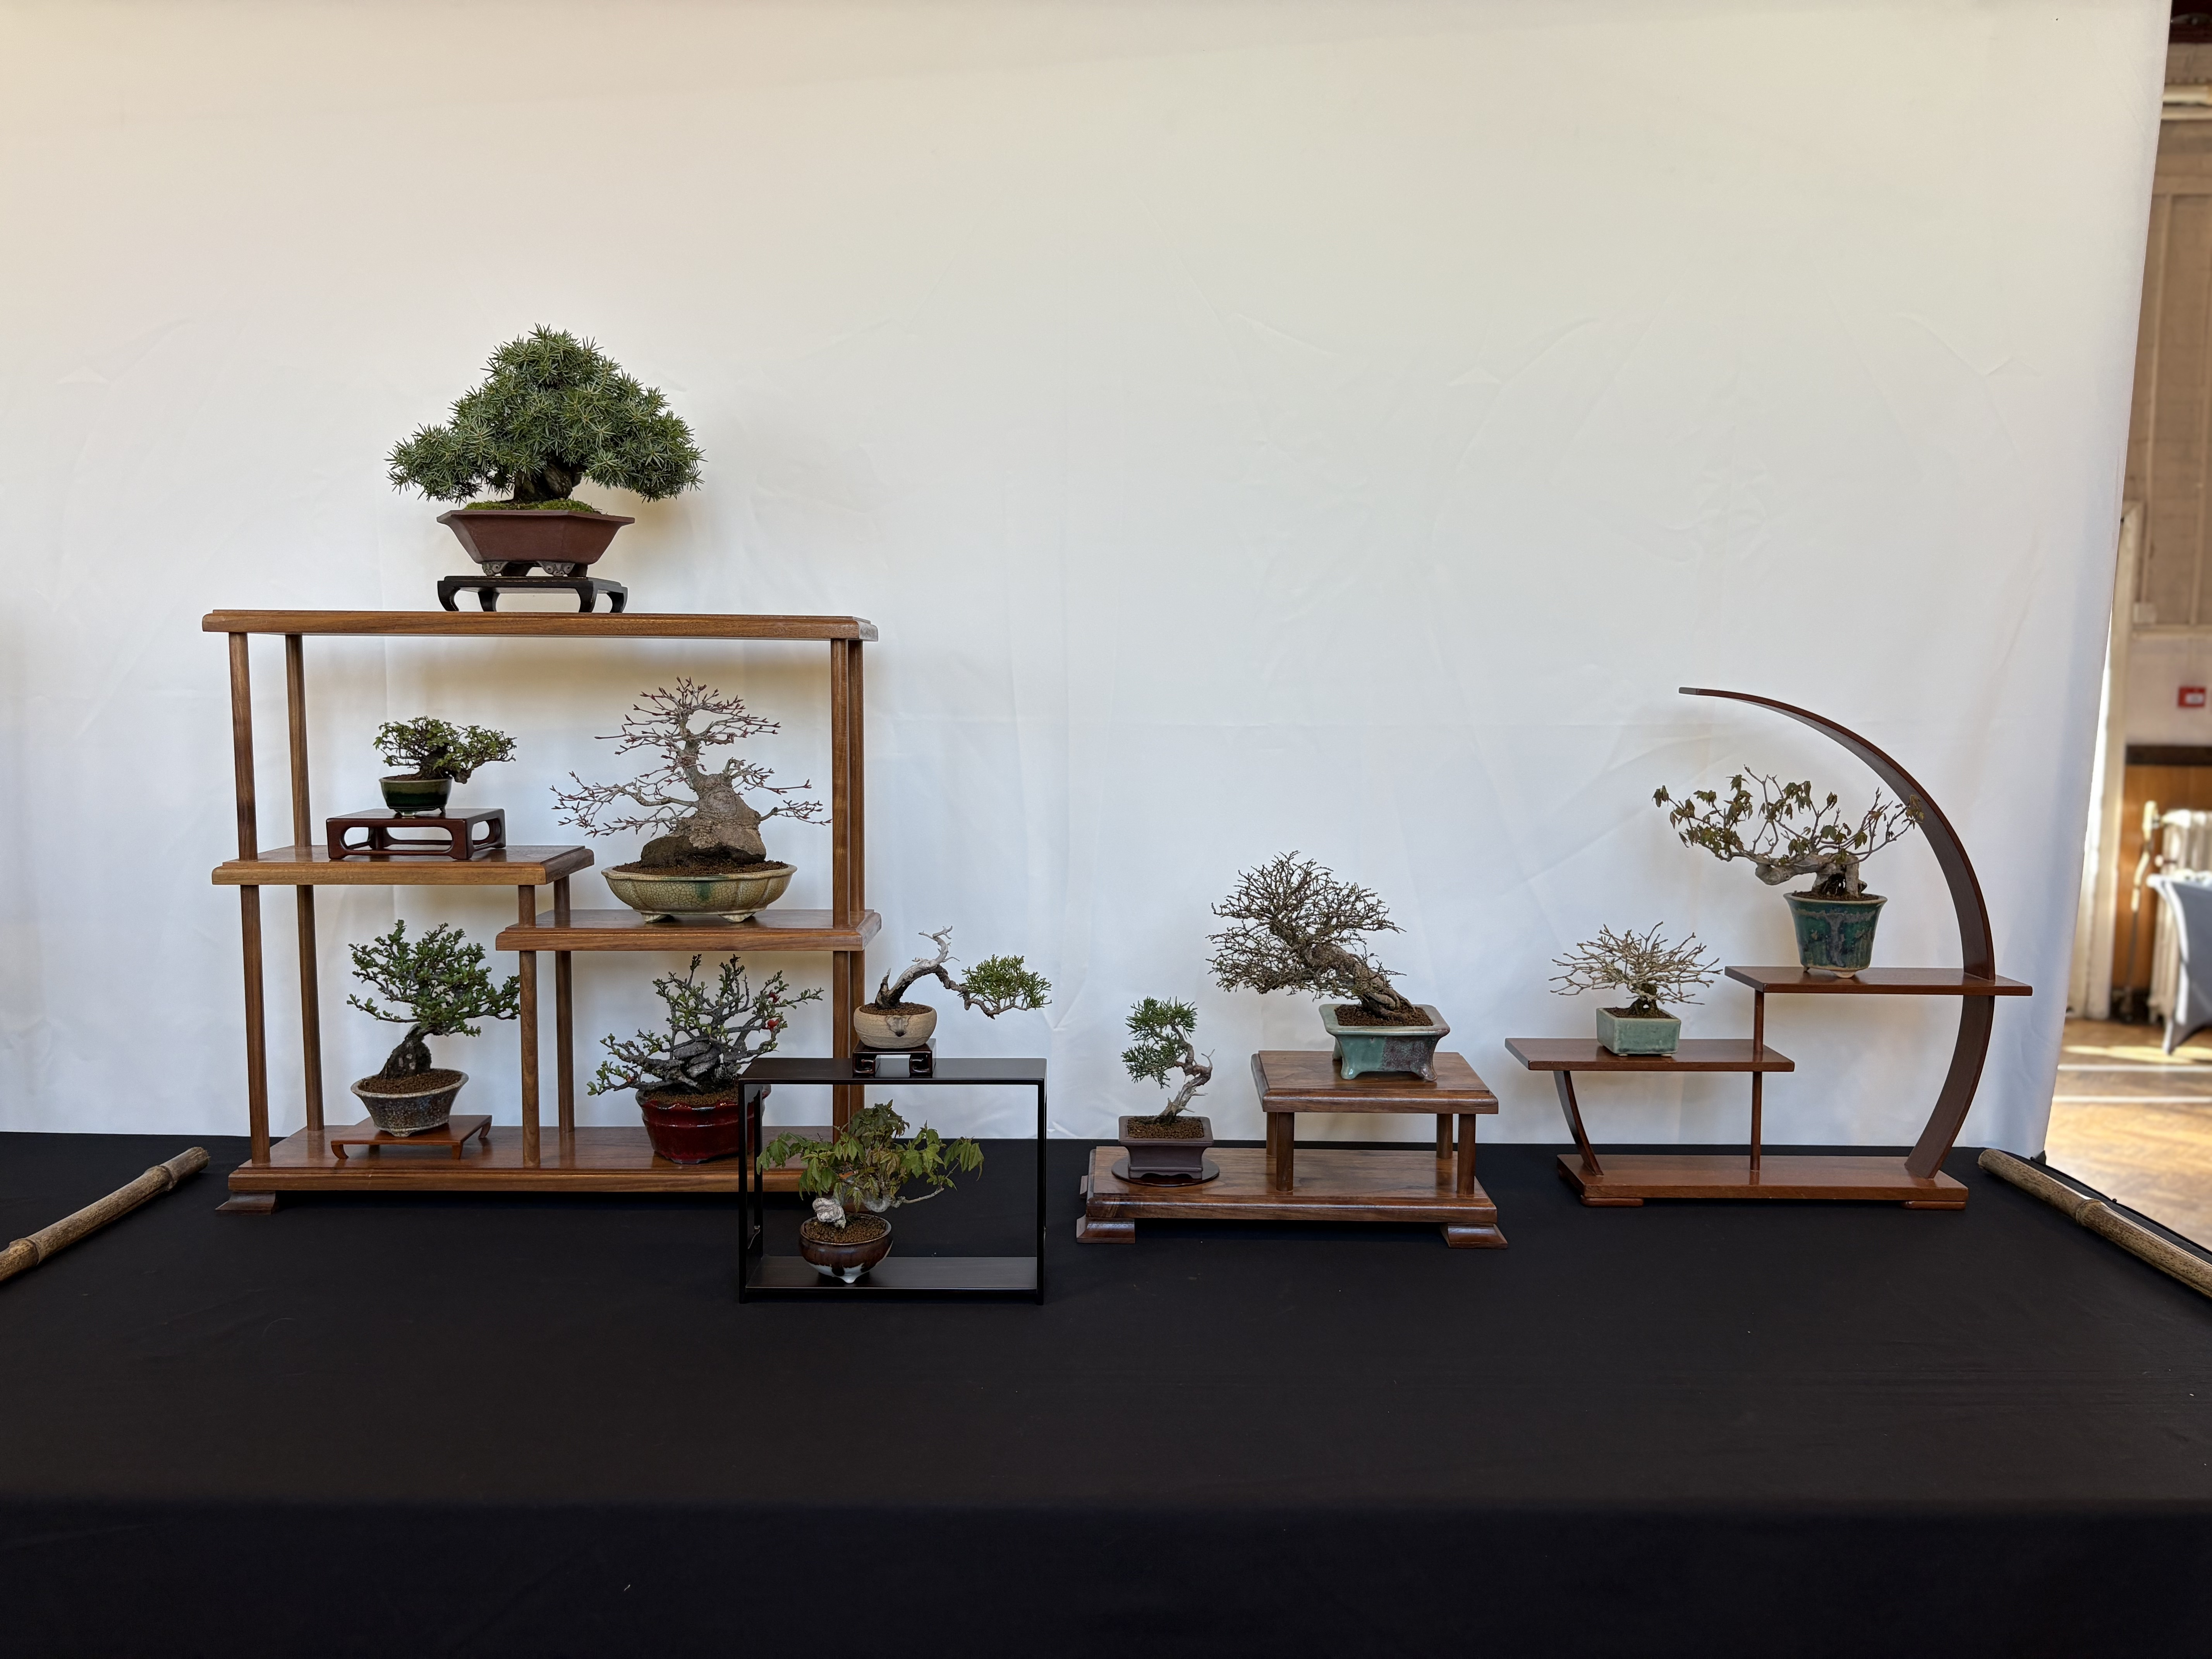
\includegraphics[width=1.0\textwidth]{2025_04/res/display_18.jpeg}
% \centerline{\emph{Mark's Hawthorn.}}
\end{minipage}
\medskip

% \begin{minipage}[b]{.42\textwidth}
% \includegraphics[width=1.0\textwidth]{2025_01/contest_stefano_benjamina.jpg}
% \centerline{\emph{Stefano's Ficus Benjamina.}}
% \end{minipage}

\centerline{%
\emph{The grand finale of petite bonsai masterpieces that stirred Chobham Village Hall.}%
}
\end{figure*}

\topic{Creating Interesting Trunks Through Grafting}
\noindent
To accelerate the development of trunks with character, David employs grafting techniques. He described how he uses San Jose junipers as a base, as they grow faster than other varieties like Itoigawa. By shaping and wiring the San Jose trunk while young and then grafting Itoigawa branches onto it, he creates visually interesting bonsai much more quickly than through traditional slow\--growing methods.

Once the Itoigawa grafts establish themselves, he removes the original San Jose foliage to ensure all the tree's energy goes into the new branches. This method allows him to produce trunks that would otherwise take decades to develop naturally.

\medskip

\begin{figure*}[!tb]
\centering
\begin{minipage}[b]{.47\textwidth}
\includegraphics[width=1.0\textwidth]{2025_04/res/principles_01.jpeg}
\end{minipage}\qquad
\begin{minipage}[b]{.47\textwidth}
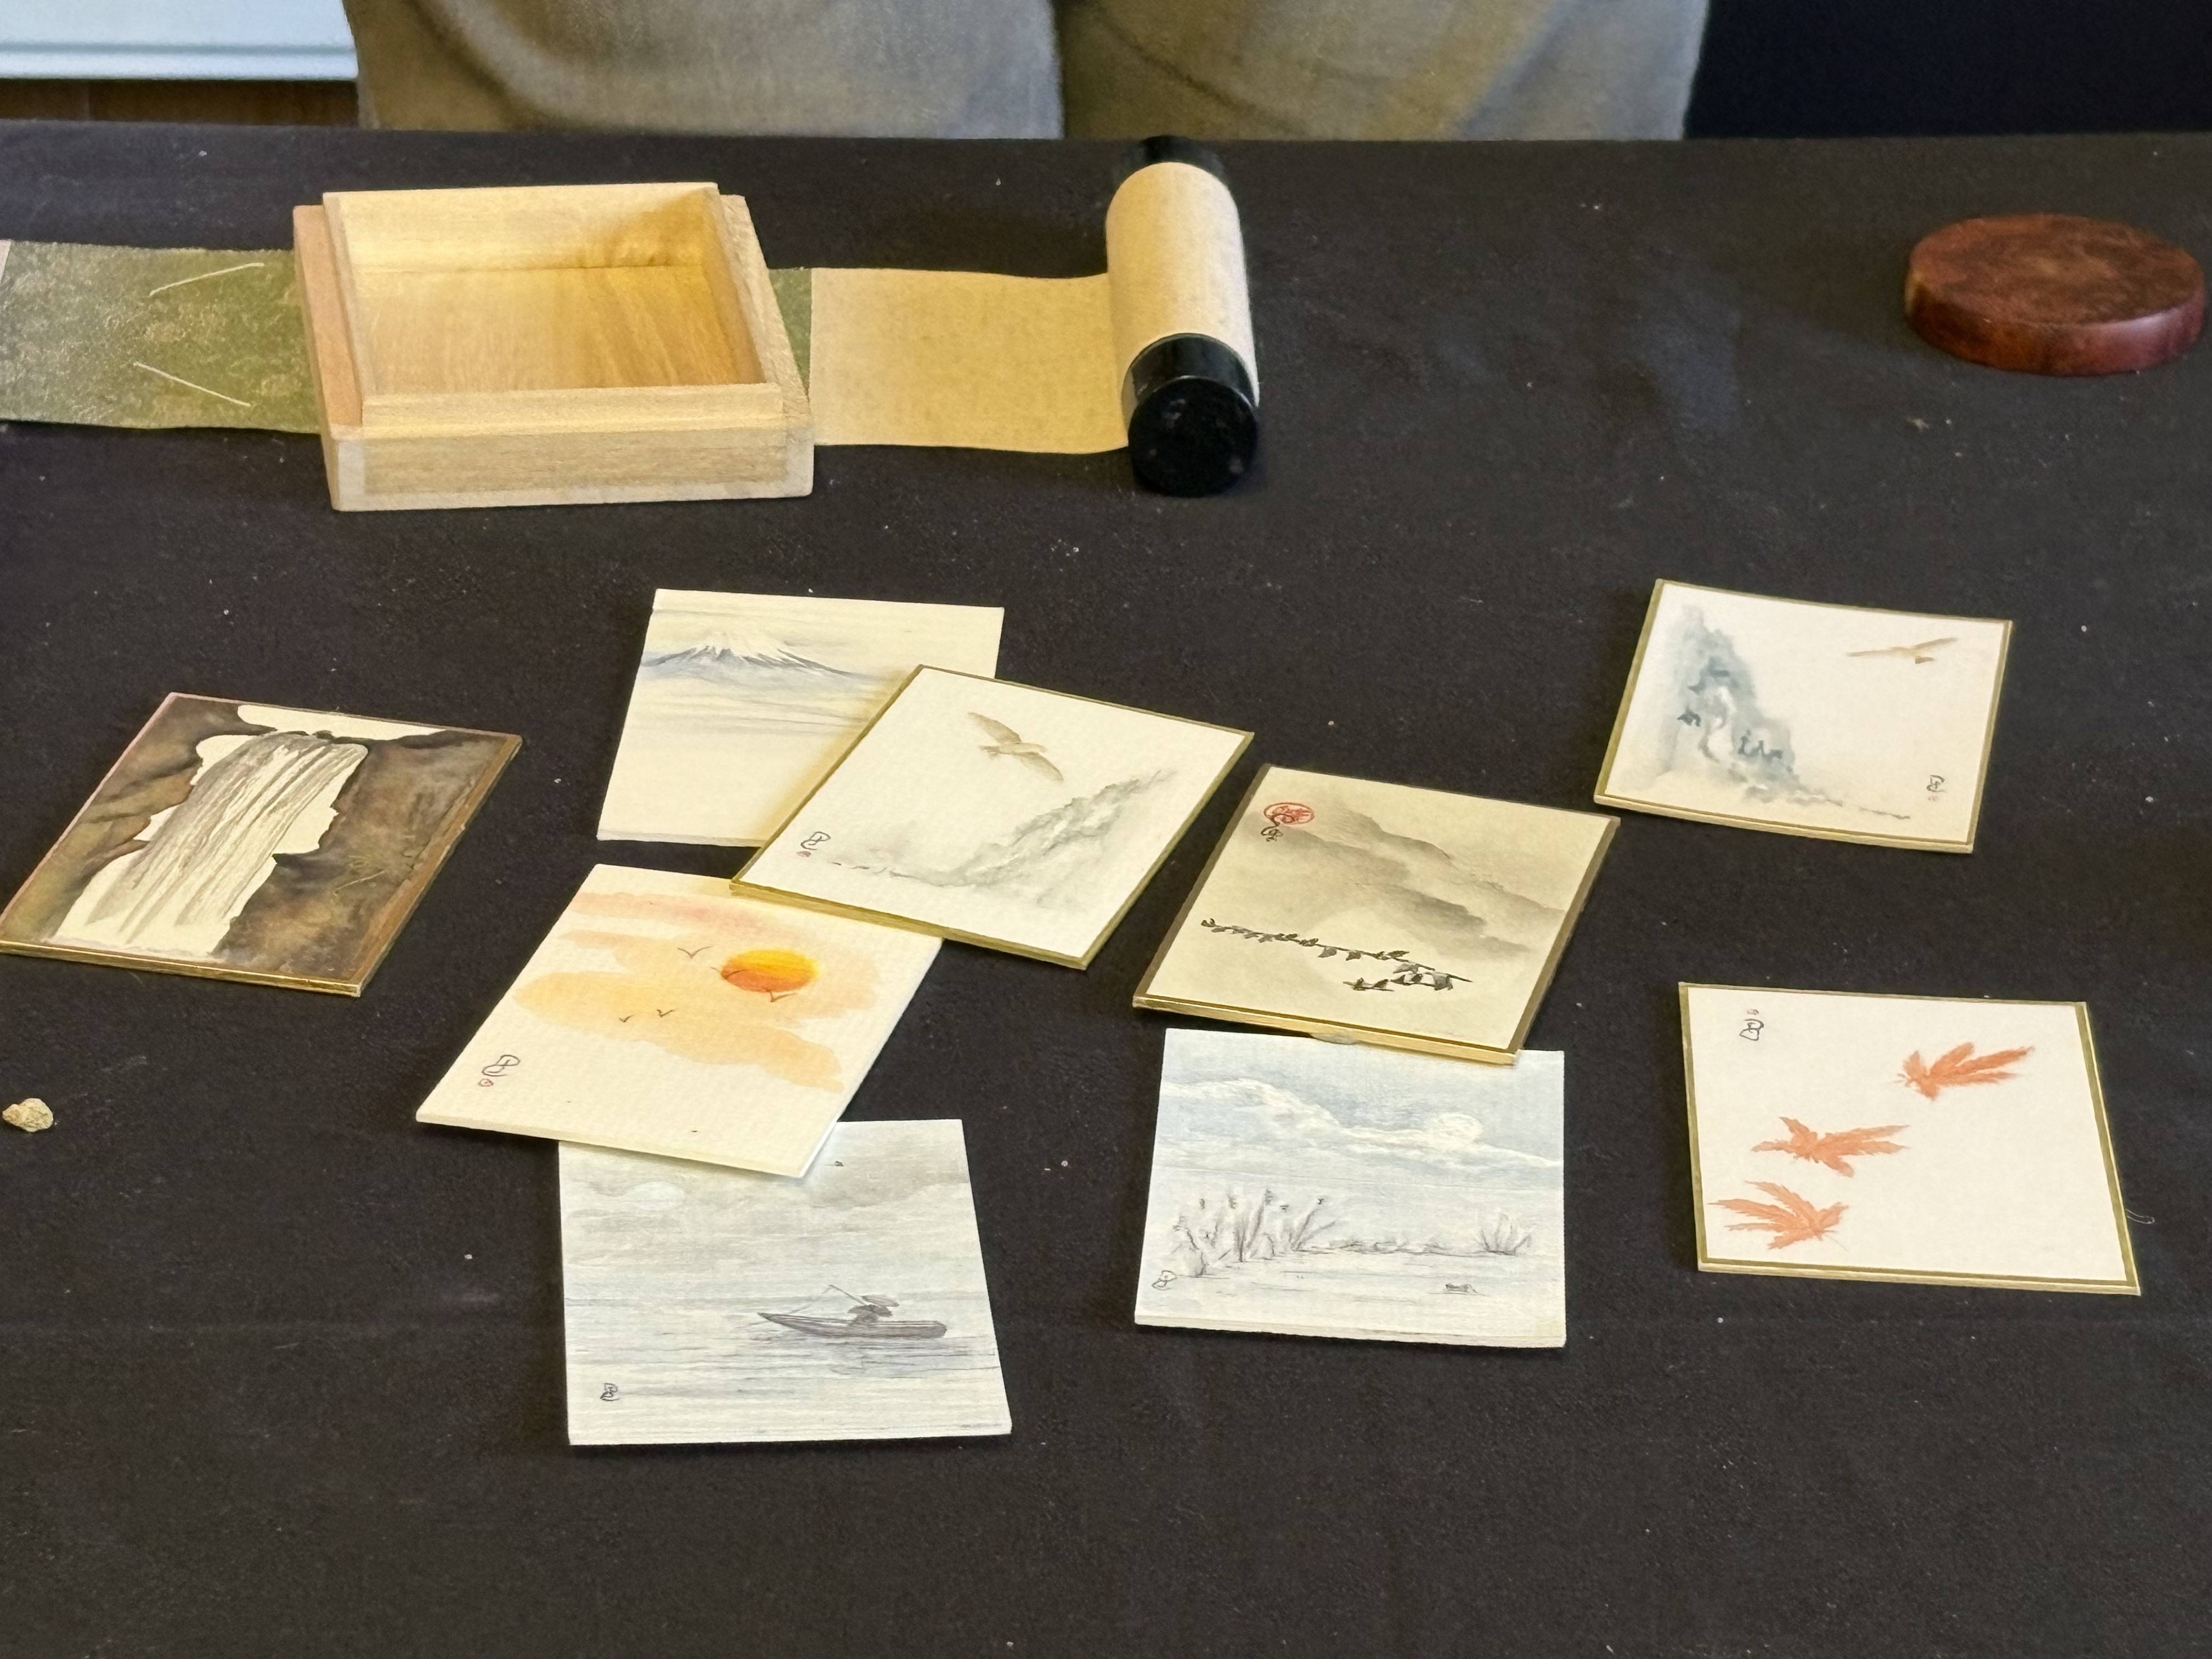
\includegraphics[width=1.0\textwidth]{2025_04/res/principles_02.jpeg}
\end{minipage}
\medskip 

\centerline{%
\emph{Gary Careford explains how to create a mini bonsai display and shares tips for selecting scroll artwork.}}
\end{figure*}

\topic{Balancing Patience with Commercial Viability}
\noindent
David acknowledged the tension between traditional slow\--growing bonsai methods and the need for commercial viability. While the Japanese approach favours long\--term development, he explores ways to speed up the process slightly without compromising quality. This includes using slightly larger pots to encourage faster growth while maintaining control over shape and structure.

Despite experimenting with these faster methods, he remains committed to the philosophy that the journey of bonsai cultivation is as important as the end result. Watching trees change through the seasons and appreciating their natural transformations is part of what makes bonsai growing so rewarding.

\medskip

\topic{The Beauty of Seasonal Change}
\noindent
David encouraged bonsai enthusiasts to embrace the seasonal changes of their trees. He noted that many growers instinctively remove yellowing pine needles in autumn, yet this colour change is a natural and beautiful part of the tree's life cycle. Instead of seeing it as a flaw, he suggested enjoying the rich autumn hues before eventually removing the old needles.

This appreciation for natural transitions is a fundamental aspect of Japanese bonsai culture, where each stage of a tree's life is valued rather than being rushed through.

\medskip

\topic{Conclusion}
\noindent
David's talk provided a deep dive into the intricacies of growing Mame bonsai, blending traditional Japanese techniques with his own practical experiences. His advice covered everything from managing climate conditions to advanced propagation techniques, offering invaluable guidance for both beginners and experienced bonsai enthusiasts. 

Above all, his message was clear: bonsai growing is a journey to be savoured. Whether through patient cultivation or careful selection of cuttings, each step in the process contributes to the beauty and artistry of bonsai.



% QWERTY












% David Cheshire (David Cheshire Nurseries) opened his talk by observing a trend among enthusiasts---moving towards smaller trees, or \textit{mame bonsai}. His interest in these miniature specimens led him to study specialised techniques in Japan, particularly from nurseries focusing on compact, naturally styled trees. He emphasised that traditional Japanese bonsai (\textit{noe\--uchi}, meaning ``natural bonsai'') prioritises slow, organic growth over the modern commercial approach, which favours rapid development and dramatic features like thick trunks.  

% The core difference lies in patience: traditional methods mimic how trees grow in harsh wild conditions---think of a seed lodged in a mountain crevice, surviving on minimal soil and water. These trees develop gnarled bark and compact forms over decades, sometimes centuries. Modern techniques, however, are designed for efficiency, often sacrificing longevity for quicker results.

% \medskip

% \topic{\large{Traditional Slow\--Growth Techniques}}
% %\noindent
% %
% %\medskip
% %
% \topic{Potting and Root Management}
% \noindent
% For \textit{mame bonsai}, David stressed starting with seedlings in \textbf{tiny pots}---no larger than a fist---for the first 5–6 years. The goal isn't vigorous growth but survival, allowing the bark to harden naturally. Repotting is done incrementally into slightly larger containers, \textbf{without root pruning}. Instead, the tree is raised higher in the pot over time, letting surface roots emerge and thicken, creating the illusion of age.  
% \medskip

% \topic{Environmental Conditioning}
% \noindent
% Trees are ``programmed'' to thrive in austerity:  

% \begin{itemize}
%     \item \textbf{Watering}: Minimal irrigation trains roots to seek moisture, preventing reliance on constant care.  

%     \item \textbf{Nutrients}: Sparingly applied to avoid lush, unsustainable growth.  
% \end{itemize}

% This mimics nature, where stunted trees outlive fast\--grown ones. A 45\--year\--old pine shown at the talk had a trunk no thicker than a pencil but displayed deeply fissured bark---proof of this method's effectiveness.  
% \medskip

% \topic{Shaping Without Wiring}
% \noindent
% Instead of wire, David demonstrated how sunlight manipulation shapes trees. For example:  
% \begin{itemize}
%     \item Tilting a pot forces branches to grow toward the light, creating movement.  
%     \item A red pine in the talk had never been wired; its curves resulted from decades of strategic repositioning.  
% \end{itemize}
% Branches are allowed to die back naturally, adding character---a stark contrast to the ``perfect'' aesthetics of modern bonsai.  

% \columnbreak

% \topic{\large{Fast\--Growth Methods and Their Trade\--Offs}}
% %\noindent
% %
% %\medskip
% %
% \topic{Sacrificial Branch Technique}
% \noindent
% For quicker results, David showcased a Japanese maple grown in coarse volcanic grit. To thicken the trunk, a \textbf{sacrificial branch} was partially removed:  

% \begin{itemize}
%     \item The underside was carved out, leaving a thin connection to draw sap.  

%     \item Once callus tissue half\--covered the wound, the branch was fully removed, ensuring smooth healing.  
% \end{itemize}

% While effective, such methods risk internal rot, limiting the tree's lifespan to 40–50 years.  

% \medskip

% \topic{Grafting for Speed}
% \noindent
% \begin{itemize}
%     \item \textbf{Vigorous Rootstock}: Fast\--growing species (e.g., \textit{San Jose juniper}) form trunks quickly.  
    
%     \item \textbf{Desired Foliage}: Slower varieties (e.g., \textit{Itoigawa juniper}) are grafted onto the established trunk.  
% \end{itemize}

% David noted that grafts must dominate early---if the rootstock's foliage isn't removed promptly, it can outcompete the grafted branches.  

% \medskip

% \topic{\large{Species\--Specific Strategies}}
% %\noindent
% %
% %\medskip
% %
% \topic{Zelkova: The Tied\--Branch Trick}
% \noindent
% Japanese elms (\textit{zelkova}) often have tightly clustered crowns in maturity. To replicate this in \textit{mame} sizes:  

% \begin{itemize}
%     \item Young branches are \textbf{bound together with wire} for months, encouraging upright growth.  
    
%     \item Once released, they retain a compact, broom\--like silhouette.  
% \end{itemize}

% \medskip

% \topic{Elms: Propagation Secrets}
% \noindent
% Elms (\textit{Almus}) excel for \textit{mame} projects due to their adaptability:  
% \begin{itemize}
%     \item \textbf{Cuttings}: Taken from older, slower\--growing side shoots (not vigorous tips) for compactness.  
    
%     \item \textbf{Winged Varieties}: Some elms develop corky bark ``wings''---David hunts for these rare traits to propagate.  
% \end{itemize}

% \medskip

% \topic{Pines: Embracing Seasonality}
% \noindent
% David urged attendees to appreciate seasonal changes:  

% \begin{itemize}
%     \item Yellowing autumn needles shouldn't be immediately plucked---their colour adds depth.  

%     \item Slow\--grown pines develop finer needles and denser foliage over time.  
% \end{itemize}

% \medskip

% \topic{\large{Climate Adaptation: UK Challenges}}
% %\noindent
% %
% %\medskip
% %
% \topic{Humidity and Watering}
% \noindent
% \begin{itemize}
%     \item \textbf{Summer}: UK air is drier than Japan's. David uses gravel trays and brief sprinkler bursts to boost humidity \textbf{without overwatering roots}.  

%     \item \textbf{Winter}: Wet cold promotes fungus. Trees are kept drier, with shelter from relentless rain.  
% \end{itemize}

% \medskip

% \topic{Light and Heat Management}
% \noindent
% Small pots heat rapidly in direct sun. Solutions:  

% \begin{itemize}
%     \item \textbf{Shade Cloth}: Filters intense midday light.  

%     \item \textbf{Grouping Trees}: Creates a self\--shading microclimate.  
% \end{itemize}

% \medskip

% \topic{\large{Nursery Practices and Personal Insights}}
% %\noindent
% %
% %\medskip
% %
% \topic{Propagation Philosophy}
% \noindent
% \begin{itemize}
%     \item \textbf{High Volume}: Grow many seedlings---expect 50\% losses, as in nature.  

%     \item \textbf{Selection}: Keep only the strongest, most adaptable trees.  
% \end{itemize}

% % \medskip

% % \topic{The ``Hidden Trees'' Dilemma}
% % \noindent
% % David joked about hiding his favourite specimens: ``If clients see them, they'll nag until you sell!'' His personal collection focuses on experimental techniques, like grafting elms onto rocks or hybridising slow/fast methods.  

% \medskip

% \topic{Conclusion: Patience as the Core Principle}
% \noindent
% Whether adopting traditional \textit{noe\--uchi} or modern shortcuts, David's message was clear: bonsai is a dialogue with nature. \textit{Mame} bonsai distills this into its purest form---where every year of patience is etched into the bark of a tree that fits in your palm.  

\closearticle
% \columnbreak
